% FUNDAMENTACAO TEORICA------------------------------------------------------------------

\chapter{FUNDAMENTAÇÃO TEÓRICA}
\label{chap:fundamentacao-teorica}Este capítulo tem por finalidade a apresentação dos aspectos teóricos e trabalhos relacionados, sendo constituído pelas seguintes seções: Seção \ref{sec:arduino}, onde será apresentada a plataforma Arduino, expondo algumas de suas características; Seção \ref{sec:engenhariaDeSoftware}, na qual serão abordados alguns conceitos de engenharia de \textit{software}. Seção \ref{subsec:testeDeSoftware}, onde será descrito o teste de \textit{software}, suas etapas e técnicas; Seção \ref{subsec:manutencaoDeSoftware}, definindo manutenção de \textit{software} e mostrando o quanto de esforço ela exige no desenvolvimento de um sistema; Seção \ref{subsec:processoDeSoftware}, na qual é descrito o processo de \textit{software}, o modelo cascata e o modelo incremental; E por fim, a seção \ref{sec:trabalhos-relacionados}, descrevendo alguns trabalhos relacionados.

\section{PLATAFORMA ARDUINO}
\label{sec:arduino} O Arduino é uma plataforma de prototipagem eletrônica \textit{open-source} criada em 2005, que baseia-se em hardware e software flexíveis e de fácil uso, tornando-se acessível para novatos e profissionais. O Arduino é capaz de perceber o estado do ambiente através de sensores e interagir com o mesmo por meio de motores e outros atuadores, isto pode ser feito enviando um conjunto de instruções para o microcontrolador através da linguagem de programação Arduino e a IDE Arduino. Por ser uma plataforma \textit{open-source}, possui uma vasta quantia de contribuições da comunidade mundial, composta por estudantes, programadores, artistas e profissionais, o que gera uma grande quantidade de conhecimento acessível, útil para usuários novatos e experientes \cite{arduino2018}.

Professores e alunos utilizam a plataforma para o desenvolvimento de instrumentos científicos de baixo custo, ou para introduzir a programação e a robótica, além de ser utilizada também por amadores, principalmente pelas seguintes características: 

\begin{itemize}
    \item \textbf{Baixo custo:} As placas são mais baratas em comparação com outros microcontroladores.
    \item \textbf{Multiplataforma:} A IDE utilizada para o desenvolvimento de um \textit{sketch} (nome dado aos programas, uma unidade de código que é carregada e executada em uma placa), chamada de Arduino Software, ´pode ser utilizada em sistemas operacionais Windows, Linux e Mac Os, diferenciando-se dos demais, limitados ao sistema operacional Windows.
    \item \textbf{ Ambiente de programação fácil e transparente:} O Arduino Software é de fácil utilização para iniciantes e adaptável o suficiente para que usuários avançados tirem um melhor proveito da plataforma.
    \item \textbf{Software \textit{open source} e flexível:} O software Arduino é uma ferramenta \textit{open source}, podendo ser modificada e aprimorada por usuários experientes. A linguagem pode ser expandida através de bibliotecas em C++, além disto, pode-se adicionar trechos de código de uma linguagem de programação estendida da linguagem C, específica para microcontroladores, direto nos programas do Arduino.
    
    \item \textbf{Hardware \textit{open source} e flexível:} os planos das placas Arduino são publicados sob uma licença Creative Commons, permitindo o aprimoramento e criação de novos módulos \cite{arduino2018}.
\end{itemize}


\section{CONCEITOS DE ENGENHARIA DE \textit{SOFTWARE}}
\label{sec:engenhariaDeSoftware}
Nesta seção, os principais conceitos de ES que serão abordados neste trabalho são discutidos nas próximas subseções.

\subsection{TESTE DE \textit{SOFTWARE}}
\label{subsec:testeDeSoftware} A computação evoluiu muito nas últimas décadas, sendo utilizada em diversas áreas da atividade humana, demandando qualidade e produtividade, e a engenharia de \textit{software} acompanhou esse progresso, estabelecendo técnicas, critérios, métodos e ferramentas para o desenvolvimento de programas. A engenharia de \textit{software} pode ser definida como uma disciplina que aplica os princípios da engenharia para a produção de sistemas de alta qualidade e baixo custo \cite{Pressman2011}. Apesar dos métodos e técnicas empregadas na produção de \textit{softwares}, ainda podem ser encontrados erros, defeitos e falhas no produto, e com o intuito de minimizar a ocorrência destes, algumas atividades são introduzidas ao longo de todo o processo de desenvolvimento, sendo o teste de \textit{software} a mais utilizada \cite{Maldonado1997}, constituindo-se em um dos elementos para oferecer evidências de confiabilidade ao sistema.

Para um melhor entendimento desta seção, serão apresentados alguns conceitos, como defeito, falha, erro e caso de teste.

\textbf{Defeito:} É uma imperfeição ou deficiência em um componente do projeto, onde o componente não atende aos seus requisitos e necessita ser consertado ou substituído \cite{PMBOK2013}.

\textbf{Falha:} É a interrupção da capacidade de um sistema para executar uma função exigida ou sua incapacidade de executar dentro dos limites especificados anteriormente \cite{ISOEC15026}.

\textbf{Erro:} Um erro pode ser a diferença entre um valor ou condição calculada, observada ou medida e o valor ou condição verdadeira, especificada ou teoricamente correta, ou ainda, o estado errôneo do sistema. \cite{ISOEC15026}

\textbf{Caso de Teste:} Um caso de teste é um conjunto de entradas de teste, condições de execução e resultados esperados, criados para atingir um objetivo em específico, como a execução de um determinado caminho do programa ou verificação da satisfação de um determinado requisito. Alguns objetivos dos casos de testes são: encontrar defeitos, criação de produtos de qualidade, verificar a precisão do produto, minimização de custos de suporte técnico e avaliação da conformidade com os requisitos. Se um teste não for realizado de maneira correta, o \textit{software} continua com os defeitos e o mesmo não tem qualidade, não atendendo às expectativas do cliente. O caso de teste desempenha um papel importante para garantir que o teste seja feito de maneira correta \cite{ieeeTestCase2014}. A Figura \ref{fig:figura-exemplo-caso-de-teste} mostra um exemplo de um caso de teste para um projeto, onde ao girar um potenciômetro, 4 LEDs alinhados devem acender sequencialmente.

\begin{figure}[!htb]
    \centering
    \caption{Exemplo de um Caso de Teste}
    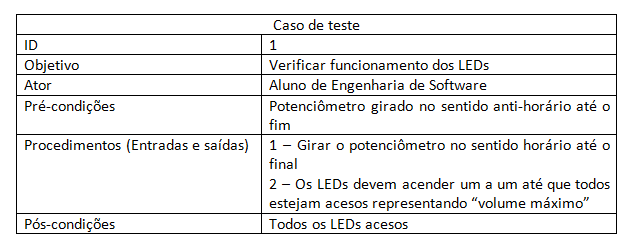
\includegraphics[width=1\textwidth]{./dados/figuras/casoDeTeste}
    \fonte{\cite{utfpr2017}}
    \label{fig:figura-exemplo-caso-de-teste}
\end{figure}

O teste de software é compostos por quatro etapas: planejamento de testes, projeto de caso de testes, execução e avaliação dos resultados dos testes, que são executadas ao longo do desenvolvimento do software e efetivam-se em três diferentes fases de teste: de unidade, de integração e de sistema. No primeiro, dedica-se na menor unidade do projeto, identificando erros de lógica e implementação em cada parte do programa. O teste de integração é realizado durante a integração da estrutura do programa, e tem como objetivo, a partir dos módulos testados no nível de unidade, construir a estrutura do programa, na forma determinada pelo projeto. O teste de sistema, é realizado após a integração do sistema, identificando erros de funções e características de desempenho que não estejam na especificação \cite{Maldonado2004}.

Os teste funcionais, conhecido como teste de caixa-preta e os testes estruturais, também chamados de teste de caixa-branca, são exemplos de técnicas de teste de software. No primeiro, não há a necessidade do testador conhecer a codificação, ele apenas informa os dados de entrada e examina se a saída está de acordo com o esperado, portanto os testes de caixa-preta visam detectar se o sistema aceita entradas incorretas, se a saída gerada está correta, se existem erros na interface e a falta de alguma funcionalidade. O segundo, observa a estrutura do código fonte para identificar a implementação e se os testes estão cobrindo diferentes caminhos, sendo assim, estes testes são implementados de forma a testar decisões logicas, variáveis estáticas, variáveis dinâmicas e \textit{loops}, por exemplo.\cite{Pedro}

A Figura \ref{fig:figura-modelo-etapas-teste-de-software} ilustra as etapas 
\begin{figure}[!htb]
    \centering
    \caption{Modelo das etapas do teste de software}
    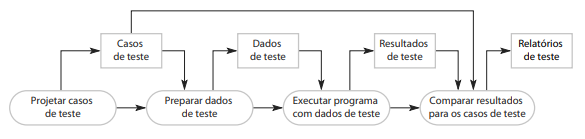
\includegraphics[width=1\textwidth]{./dados/figuras/Modelo_processo_de_software}
    \fonte{\cite{iansommerville}}
    \label{fig:figura-modelo-etapas-teste-de-software}
\end{figure}



\subsection{MANUTENÇÃO DE SOFTWARE}
\label{subsec:manutencaoDeSoftware}

A vida de um \textit{software} não é finalizada após a sua implementação. Ele ainda será utilizado por muito tempo, e passará por muitas atualizações, tanto para correção de erros ou apenas para otimização. Essa fase do processo de desenvolvimento de software é denominada manutenção de software. Este é um procedimento de melhoria de um programa que está em desenvolvimento ou já foi desenvolvido, ou seja, já está em ambiente de produção. Com a manutenção, também é realizado a correção dos erros encontrados por usuários do sistema ou testes realizados por desenvolvedores \cite{rodrigoSpinola2011}.

Existem diversas razões para que um software sofra alterações, principalmente se este implementar soluções aproximadas para problemas do mundo real. Uma destas razões, é por exemplo, o passar do tempo e o aumento da familiaridade com problema. Conforme o melhor entendimento do problema, pode-se encontrar uma melhor solução para o mesmo, acarretando uma modificação em partes ou todo o sistema. Alguns outros motivos para a ocorrência de alterações são: a mudança de legislações na qual o sistema foi baseado, fazendo com que seja necessário modificações para atender a legislação em vigor. Novos requisitos do cliente, que surgiram com a utilização do sistema. Ou ainda, devido a forma inesperada de utilização do software pelos usuários.

----- (professor pediu para melhorar aqui) A manutenção de software pode ser dividida em diferentes tipos, segundo \cite{iansommerville} é dividida em 3 tipos: ---------


\begin{itemize}
    \item \textbf{Manutenção Corretiva:} Correção de erros que não foram detectados na fase de teste, que podem não atrapalhar o funcionamento do software, sendo corrigidos por simples reparações, ou defeitos mais complexos, que exijam uma manutenção temporária, com o objetivo de manter o funcionamento normal do software e posteriormente disponibilizar uma correção definitiva em uma nova versão. 
\end{itemize}
    
\begin{itemize}  
    \item \textbf{Manutenção Adaptativa:} Adequação do software em relação as mudanças ocorridas no ambiente externo, que podem ser mudanças na regra de negócio, novos sistemas operacionais que não sejam compatível com o software, nova plataforma de hardware ou mudanças na constituição e leis que afetam funções do sistema.
\end{itemize}
    
 \begin{itemize}  
    \item \textbf{Manutenção Evolutiva (Perfectiva):} Melhorar a qualidade do software, com modificações que não estavam previstas no documento de requisitos original do projeto, através da adição de novas funcionalidades, para obter um melhor desempenho ou a modificação do código para a adaptação a algum paradigma de programação. 
\end{itemize}
    
A manutenção ocupa uma maior parte nos orçamentos de tecnologia da informação se comparado ao desenvolvimento, aproximadamente dois terços do orçamento, sendo a maioria destes para a implementação de novos requisitos do que na correção de \textit{bugs}. A \autoref{fig:figura-distribuicao-esforco} apresenta, de forma aproximada, a distribuição dos custos de manutenção. Dedicar esforços no projeto e implementação de um sistema, tornando-o mais compreensível e de fácil manutenção, pode reduzir os custos de futuras alterações. Boas práticas de engenharia de software e a utilização de desenvolvimento orientado a objeto, auxiliam para alcançar esta redução \cite{iansommerville}.
\begin{figure}[!htb]
    \centering
    \caption{Distribuição do esforço de manutenção}
    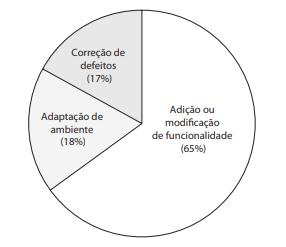
\includegraphics[width=0.5\textwidth]{./dados/figuras/distribuicao_do_esforco_de_manutencao}
    \fonte{\cite{iansommerville}}
    \label{fig:figura-distribuicao-esforco}
\end{figure}



\subsection{PROCESSO DE SOFTWARE}
\label{subsec:processoDeSoftware}

Segundo \citeonline{iansommerville}, um processo de \textit{software} é um conjunto de atividades que levam à geração de um produto de \textit{software}, onde o desenvolvimento pode dar-se a partir do zero, mas atualmente não é o que acontece, sendo eles produzidos por meio da extensão e modificação de sistemas existentes ou integração de componentes de sistemas. Para que um \textit{software} seja desenvolvido de maneira consistente, é necessário aliar um eficiente processo de \textit{software} com boas práticas de ES. Os processos de \textit{software} são complexos e necessitam de pessoas para tomarem decisões e realizarem julgamentos. Não há um processo de desenvolvimento ideal, cada sistema possui sua particularidade e deve-se escolher o processo que se adeque a ele e ao time que irá desenvolvê-lo. 

Diferentes processos de \textit{software} podem ser encontrados na literatura, mas para \citeonline{iansommerville} eles devem conter quatro atividades fundamentais para a ES:

\begin{itemize}
    \item \textbf{Especificação de \textit{software}:} A funcionalidade do \textit{software} e as restrições a seu funcionamento devem ser definidas.
    \item \textbf{Projeto e implementação de \textit{software}:} O sistema deve ser desenvolvido para respeitar as exigências do cliente. 
    \item \textbf{Validação de \textit{software}:} O sistema deve passar por uma validação para assegurar que sejam respeitadas as exigências do cliente.
    \item \textbf{Evolução de \textit{software}:} A evolução do sistema deve ocorrer para suprir a necessidade de mudança dos clientes. 
\end{itemize}


Os processos sofrem evoluções para que atinjam um melhor proveito do time de desenvolvimento, e também atender as especificidades de cada sistema. Segundo \cite{iansommerville}, os processos são categorizados em duas formas:

\begin{itemize}
    \item \textbf{Processos dirigidos a planos:} São planejadas com antecedência todas as atividades que serão realizadas, e a avaliação do projeto ocorre a partir da comparação com o planejamento feito inicialmente. Ideais para sistemas que precisam de uma análise rigorosa dos requisitos.
    \item \textbf{Processos ágeis:} Concebidos para a produção de \textit{softwares} úteis, de forma rápida, pois o planejamento acontece de forma gradativa, e pode-se facilmente realizar alterações para atender as necessidades dos clientes, devido a implementação ocorrer de forma incremental. Ideais para sistemas suscetíveis à rápidas mudanças.
\end{itemize}


Um modelo de processo é a representação do processo de \textit{software} de forma simplificada, fornecendo uma visão específica do processo, contendo apenas informações parciais. \cite{Pressman2011} cita alguns modelos de processos genéricos, que serão apresentados abaixo, que podem ser adaptados para criação de outros processos de ES para atender determinado desenvolvimento.

O modelo de processo em cascata é um exemplo de processo dirigido a plano. Nele há a necessidade de uma programação e planejamento das atividades antes de iniciar a execução. É intitulado cascata devido ao encadeamento de uma fase e outra. O modelo em cascata deve ser utilizado apenas quando os requisitos são muito bem compreendidos e não esteja sujeito a grandes alterações durante a implementação. 

\begin{figure}[!htb]
    \centering
    \caption{Modelo em Cascata}
    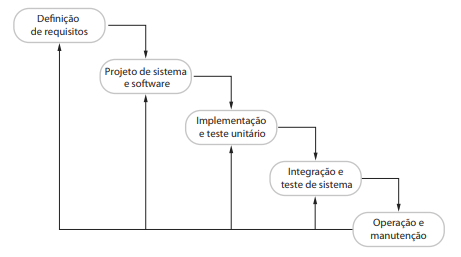
\includegraphics[width=0.8\textwidth]{./dados/figuras/modeloEmCascata}
    \fonte{\cite{iansommerville}}
    \label{fig:figura-modelo-cascata}
\end{figure}

A \autoref{fig:figura-modelo-cascata} ilustra as fases do modelo em cascata, estas refletem diretamente as principais atividades do desenvolvimento:

\begin{enumerate}
    \item \textbf{Definição dos requisitos:} Nesta fase é feito um levantamento das restrições e objetivos do produto, através de uma consulta aos clientes, posteriormente, os requisitos são estabelecidos de forma adequada para serem úteis para a próxima fase.
    \item \textbf{Projeto de sistemas e software:} Os requisitos são alocados aos sistemas e apresentados de maneira a possibilitar a codificação do produto.
    \item \textbf{Implementação e teste unitário:} Esta etapa consiste no desenvolvimento do programa, através de unidades do mesmo e a criação e execução de testes nestas unidades, para verificar se elas atendem suas especificações. 
    \item \textbf{Integração e teste de sistema:} Após o desenvolvimento de todas as unidades do programa, estas são integradas e testadas como o sistema num todo, garantindo que os requisitos do sistema foram obedecidos, mesmo após a integração, e por fim, é entregue ao cliente.
    \item \textbf{Operação e manutenção:} Considerada a fase mais longa de todo o ciclo de vida e a que mais demanda esforços, como visto na \autoref{subsec:manutencaoDeSoftware}, aqui acontece a correção de erros que só foram detectados após o uso do sistema, e a modificação, com a descoberta de novos requisitos, implicando na repetição de fases anteriores do modelo. 
\end{enumerate}


Um outro modelo de processo de \textit{software} é o modelo de desenvolvimento incremental. Este é uma abordagem ideal para sistemas de negócio e fundamental para abordagens ágeis. Ele reflete como o ser humano resolve um problema, encontrando uma solução a cada passo e recuando quando um erro é encontrado, tornando mais barato e mais fácil a realização de uma mudança durante o seu desenvolvimento. As funcionalidades neste modelo são acrescentadas em cada incremento ou nova versão, sendo as de maior importância incluídas inicialmente, possibilitando o cliente avaliar se o sistema está obedecendo o que foi solicitado. Caso ocorra alguma divergência, apenas o incremento em fase de desenvolvimento será alterado.

\begin{figure}[!htb]
    \centering
    \caption{Modelo Incremental}
    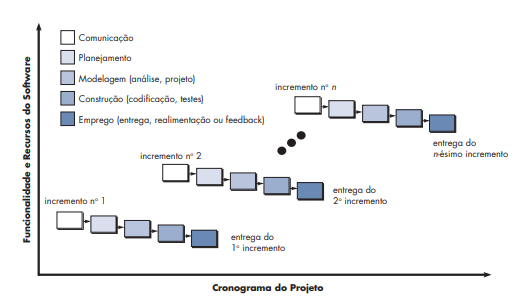
\includegraphics[width=1\textwidth]{./dados/figuras/modeloIncremental}
    \fonte{\cite{Pressman2011}}
    \label{fig:figura-modelo-incremental}
\end{figure}